\section{Model3DRigid\-Helical  Class Reference}
\label{class_Model3DRigidHelical}\index{Model3DRigidHelical@{Model3DRigid\-Helical}}
A rigid robot that moves along helical paths in a 3D world. 


{\tt \#include $<$modelnew.h$>$}

Inheritance diagram for Model3DRigid\-Helical::\begin{figure}[H]
\begin{center}
\leavevmode
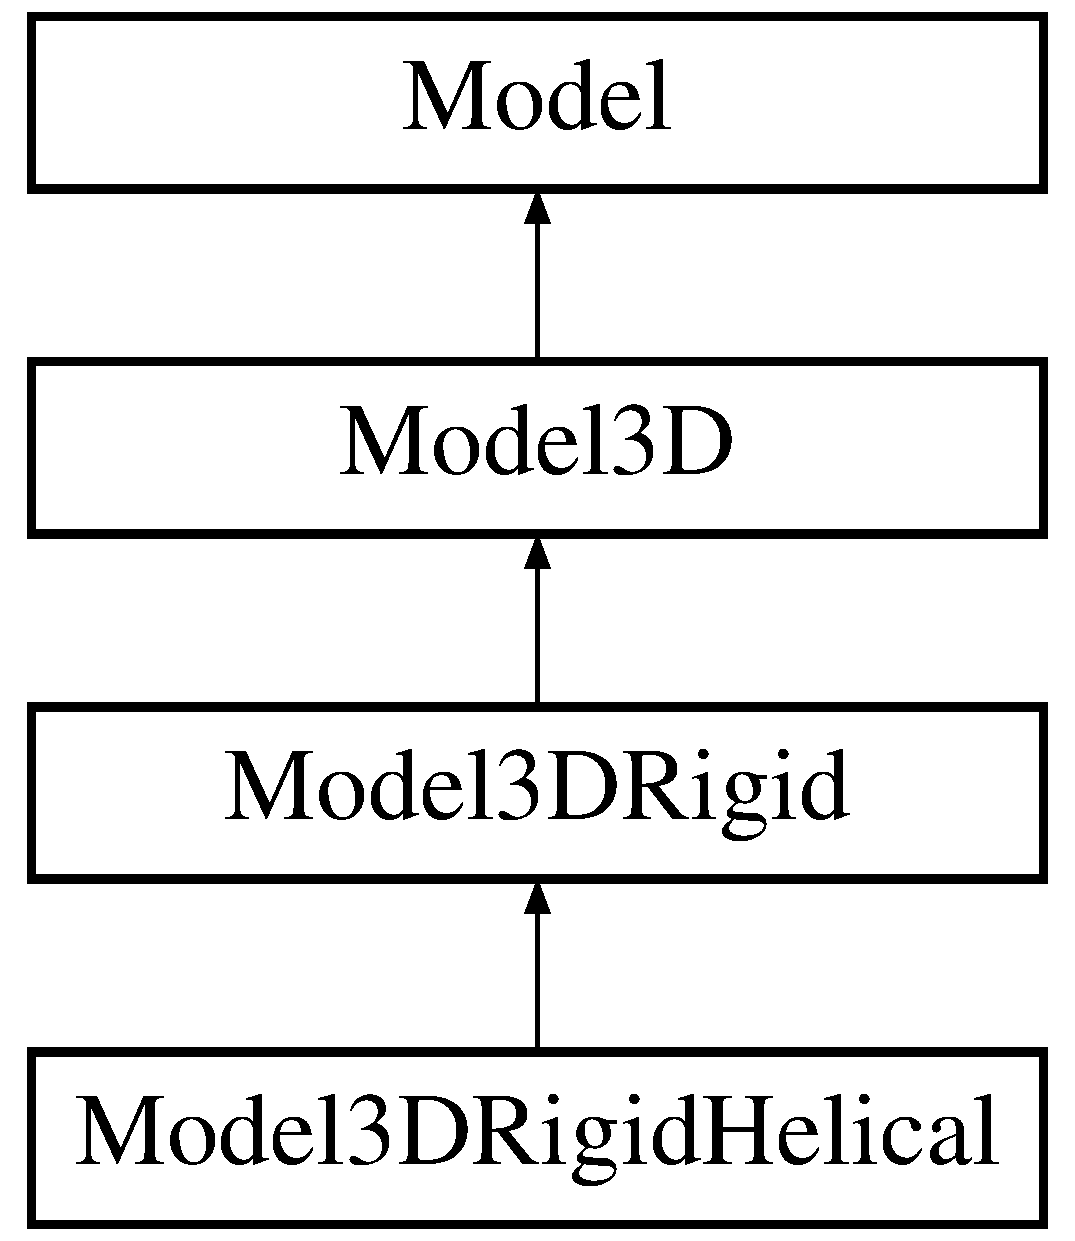
\includegraphics[height=4cm]{class_Model3DRigidHelical}
\end{center}
\end{figure}
\subsection*{Public Methods}
\begin{CompactItemize}
\item 
{\bf Model3DRigid\-Helical} (string path)
\item 
virtual {\bf $\sim$Model3DRigid\-Helical} ()
\item 
virtual {\bf MSLVector} {\bf State\-Transition\-Equation} (const {\bf MSLVector} \&x, const {\bf MSLVector} \&u)
\begin{CompactList}\small\item\em Give the equations of motion for a helical kinematic system.\item\end{CompactList}\item 
virtual {\bf MSLVector} {\bf Integrate} (const {\bf MSLVector} \&x, const {\bf MSLVector} \&u, const double \&h)
\begin{CompactList}\small\item\em Perform integration from state x, using input u, over time step h.\item\end{CompactList}\end{CompactItemize}


\subsection{Detailed Description}
A rigid robot that moves along helical paths in a 3D world.



\subsection{Constructor \& Destructor Documentation}
\index{Model3DRigidHelical@{Model3DRigid\-Helical}!Model3DRigidHelical@{Model3DRigidHelical}}
\index{Model3DRigidHelical@{Model3DRigidHelical}!Model3DRigidHelical@{Model3DRigid\-Helical}}
\subsubsection{\setlength{\rightskip}{0pt plus 5cm}Model3DRigid\-Helical::Model3DRigid\-Helical (string {\em path})}\label{class_Model3DRigidHelical_a0}


\index{Model3DRigidHelical@{Model3DRigid\-Helical}!~Model3DRigidHelical@{$\sim$Model3DRigidHelical}}
\index{~Model3DRigidHelical@{$\sim$Model3DRigidHelical}!Model3DRigidHelical@{Model3DRigid\-Helical}}
\subsubsection{\setlength{\rightskip}{0pt plus 5cm}Model3DRigid\-Helical::$\sim$Model3DRigid\-Helical ()\hspace{0.3cm}{\tt  [inline, virtual]}}\label{class_Model3DRigidHelical_a1}




\subsection{Member Function Documentation}
\index{Model3DRigidHelical@{Model3DRigid\-Helical}!Integrate@{Integrate}}
\index{Integrate@{Integrate}!Model3DRigidHelical@{Model3DRigid\-Helical}}
\subsubsection{\setlength{\rightskip}{0pt plus 5cm}virtual {\bf MSLVector} Model3DRigid\-Helical::Integrate (const {\bf MSLVector} \& {\em x}, const {\bf MSLVector} \& {\em u}, const double \& {\em h})\hspace{0.3cm}{\tt  [virtual]}}\label{class_Model3DRigidHelical_a3}


Perform integration from state x, using input u, over time step h.



Reimplemented from {\bf Model3DRigid} {\rm (p.\,\pageref{class_Model3DRigid_a2})}.\index{Model3DRigidHelical@{Model3DRigid\-Helical}!StateTransitionEquation@{StateTransitionEquation}}
\index{StateTransitionEquation@{StateTransitionEquation}!Model3DRigidHelical@{Model3DRigid\-Helical}}
\subsubsection{\setlength{\rightskip}{0pt plus 5cm}{\bf MSLVector} Model3DRigid\-Helical::State\-Transition\-Equation (const {\bf MSLVector} \& {\em x}, const {\bf MSLVector} \& {\em u})\hspace{0.3cm}{\tt  [virtual]}}\label{class_Model3DRigidHelical_a2}


Give the equations of motion for a helical kinematic system.



Reimplemented from {\bf Model3DRigid} {\rm (p.\,\pageref{class_Model3DRigid_a3})}.

The documentation for this class was generated from the following files:\begin{CompactItemize}
\item 
{\bf modelnew.h}\item 
{\bf modelnew.C}\end{CompactItemize}
